\section{Date: 2026-11-15}
\noindent \textbf{Series ID: OCM2MA} 

\noindent This series is titled Real User Cost Index of MSI-M2M (alternative) and has a frequency of Monthly. The units are Percent and the seasonal adjustment is Not Seasonally Adjusted.The observation start date is 1967-01-01 and the observation end date is 2013-12-01.The popularity of this series is 1. \\ 

\noindent \textbf{Series ID: G17MVSFWAUTOS} 

\noindent This series is titled Weekday-Basis Seasonal Factors: Auto Production and has a frequency of Monthly. The units are Seasonal Factor and the seasonal adjustment is Not Seasonally Adjusted.The observation start date is 1996-01-01 and the observation end date is 2027-09-01.The popularity of this series is 2. \\ 

\subsection{Raw Regression}
\noindent Regresses the two series against each other directly. A significant result here can come just as easily from both series sharing a long-run trend as from any real relationship.

\begin{center}
\begin{tabular}{lclc}
\toprule
\textbf{Dep. Variable:}      & value\_fred\_G17MVSFWAUTOS & \textbf{  R-squared:         } &     0.000   \\
\textbf{Model:}              &            OLS             & \textbf{  Adj. R-squared:    } &    -0.004   \\
\textbf{Method:}             &       Least Squares        & \textbf{  F-statistic:       } &   0.04277   \\
\textbf{Date:}               &      Sun, 15 Nov 2026      & \textbf{  Prob (F-statistic):} &    0.836    \\
\textbf{Time:}               &          18:04:14          & \textbf{  Log-Likelihood:    } &   -854.49   \\
\textbf{No. Observations:}   &              216           & \textbf{  AIC:               } &     1713.   \\
\textbf{Df Residuals:}       &              214           & \textbf{  BIC:               } &     1720.   \\
\textbf{Df Model:}           &                1           & \textbf{                     } &             \\
\textbf{Covariance Type:}    &         nonrobust          & \textbf{                     } &             \\
\bottomrule
\end{tabular}
\begin{tabular}{lcccccc}
                             & \textbf{coef} & \textbf{std err} & \textbf{t} & \textbf{P$> |$t$|$} & \textbf{[0.025} & \textbf{0.975]}  \\
\midrule
\textbf{const}               &     101.2451  &        7.205     &    14.052  &         0.000        &       87.044    &      115.447     \\
\textbf{value\_fred\_OCM2MA} &     -25.5025  &      123.317     &    -0.207  &         0.836        &     -268.574    &      217.568     \\
\bottomrule
\end{tabular}
\begin{tabular}{lclc}
\textbf{Omnibus:}       & 56.285 & \textbf{  Durbin-Watson:     } &    2.083  \\
\textbf{Prob(Omnibus):} &  0.000 & \textbf{  Jarque-Bera (JB):  } &   92.369  \\
\textbf{Skew:}          & -1.473 & \textbf{  Prob(JB):          } & 8.76e-21  \\
\textbf{Kurtosis:}      &  4.259 & \textbf{  Cond. No.          } &     143.  \\
\bottomrule
\end{tabular}
%\caption{OLS Regression Results}
\end{center}

Notes: \newline
 [1] Standard Errors assume that the covariance matrix of the errors is correctly specified.

\begin{figure}
\centering
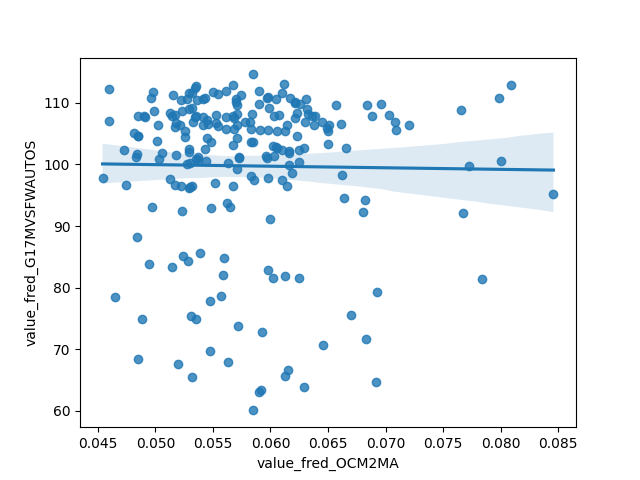
\includegraphics[scale = 0.9]{plots/plot_2026-11-15.png}
\caption{Raw Regression Plot for 2026-11-15}
\end{figure}
\newpage
\subsection{Detrended Regression}
\noindent Regresses the residuals of each series after removing its own linear time trend, so a shared trend can no longer drive the result on its own. A relationship that stays significant here is better evidence of a genuine link between the two series.

\begin{center}
\begin{tabular}{lclc}
\toprule
\textbf{Dep. Variable:}                 & value\_fred\_G17MVSFWAUTOS\_detrended & \textbf{  R-squared:         } &     0.000   \\
\textbf{Model:}                         &                  OLS                  & \textbf{  Adj. R-squared:    } &    -0.004   \\
\textbf{Method:}                        &             Least Squares             & \textbf{  F-statistic:       } &   0.04156   \\
\textbf{Date:}                          &            Sun, 15 Nov 2026           & \textbf{  Prob (F-statistic):} &    0.839    \\
\textbf{Time:}                          &                18:04:14               & \textbf{  Log-Likelihood:    } &   -854.47   \\
\textbf{No. Observations:}              &                    216                & \textbf{  AIC:               } &     1713.   \\
\textbf{Df Residuals:}                  &                    214                & \textbf{  BIC:               } &     1720.   \\
\textbf{Df Model:}                      &                      1                & \textbf{                     } &             \\
\textbf{Covariance Type:}               &               nonrobust               & \textbf{                     } &             \\
\bottomrule
\end{tabular}
\begin{tabular}{lcccccc}
                                        & \textbf{coef} & \textbf{std err} & \textbf{t} & \textbf{P$> |$t$|$} & \textbf{[0.025} & \textbf{0.975]}  \\
\midrule
\textbf{const}                          &    8.005e-12  &        0.864     &  9.26e-12  &         1.000        &       -1.703    &        1.703     \\
\textbf{value\_fred\_OCM2MA\_detrended} &     -25.1448  &      123.335     &    -0.204  &         0.839        &     -268.252    &      217.962     \\
\bottomrule
\end{tabular}
\begin{tabular}{lclc}
\textbf{Omnibus:}       & 56.027 & \textbf{  Durbin-Watson:     } &    2.084  \\
\textbf{Prob(Omnibus):} &  0.000 & \textbf{  Jarque-Bera (JB):  } &   91.685  \\
\textbf{Skew:}          & -1.470 & \textbf{  Prob(JB):          } & 1.23e-20  \\
\textbf{Kurtosis:}      &  4.244 & \textbf{  Cond. No.          } &     143.  \\
\bottomrule
\end{tabular}
%\caption{OLS Regression Results}
\end{center}

Notes: \newline
 [1] Standard Errors assume that the covariance matrix of the errors is correctly specified.

\begin{figure}
\centering
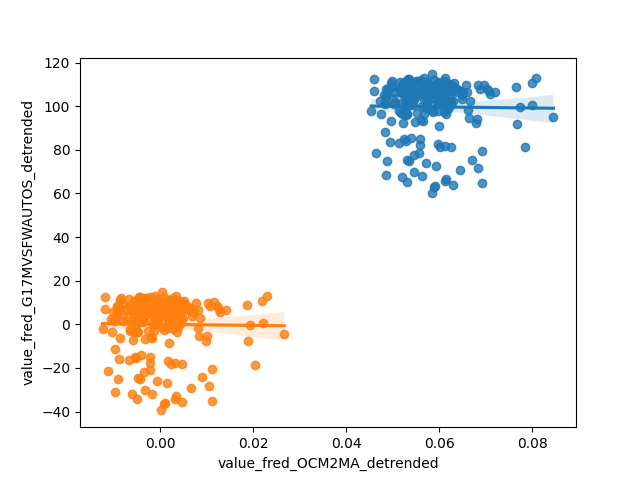
\includegraphics[scale = 0.9]{plots/plot_2026-11-15_detrended.png}
\caption{Detrended Regression Plot for 2026-11-15}
\end{figure}
\newpage
